\documentclass[notitlepage]{article}
\usepackage{amsmath,graphicx}
\usepackage[citestyle=numeric,backend=bibtex]{biblatex}
\usepackage[font=small,labelfont=bf]{caption}
\usepackage{verbatim}
\usepackage{pgfplotstable}
\usepackage[textsize=small]{todonotes}
\usepackage{soul}
\usepackage{float}
\newcommand{\hlfix}[2]{\texthl{#1}\todo{#2}}

\bibliography{library}

\title{Interim report}
\author{Uri Barenholz}

\begin{document}
\maketitle

\abstract{
Microorganisms are highly adaptable, self replicating, chemical processing machines.
A huge body of work has characterized many of their internal components, and the processes through which they proliferate.
Despite the vast knowledge obtained for these creatures, our understanding of many basic questions regarding their ability to dynamically adjust their physiology to changing environmental conditions is still far from complete.
While essential knowledge on the extent to which cell size and macromolecular composition change as a function of the environmental conditions and the growth rate has been collected for decades, quantifying  and characterizing the variability of the proteome composition has only started being addressed in recent years.
Specifically, the amount of degrees of freedom a cell has for controlling its expression program is not well known.
Furthermore, how much of the observed adaptation is due to active regulation of the expression program of the cell and how much is a passive, inevitable, global side-effect of that active regulation is not yet fully understood.

Here we present an extensive analysis of two proteomics data sets collected for the model organism \emph{E.Coli} under various environmental conditions.
Our analysis focuses on changes in the proteome that are correlated with the growth rate.
We find that the concentrations of between a third and a half of the proteins increase with the growth rate.
We describe a model that explains why the observed phenomena can result from basic physiological considerations, under some trivial assumptions.
We show that, despite the magnitude of this phenomena, it only accounts for $\approx 10 \%$ of the variability observed in the proteome in these data sets.

We are currently building a turbidostat/chemostat system that will be used to collect further data on the proteome composition under different growth rates and nutrient types.
We plan on using this data to re-evaluate our current model as well as address questions regarding the physiological changes occurring under varying nutrient concentrations and the rigidity of the transcriptome/proteome relation.
}
\section{Results}
\subsection{Analysis of proteomic data sets}
To examine the interdependence of protein concentration and growth rate across expressed genes we analyzed two proteomics data sets of \emph{E.coli}, \cite{Valgepea2013} and [ref Heinemann].
These data sets use mass spectrometry to evaluate the proteomic composition of \emph{E.coli} under $5$ different growth rates using a chemostat, in \cite{Valgepea2013}, and $19$ different growth conditions, spanning both different carbon sources and chemostat-controlled growth rates, in [ref Heinemann].
The [ref Heinemann] data set contains more conditions than those analyzed below, see section \ref{heinemanncond} for further details.
\subsubsection{A large fraction of the proteome is positively correlated with growth rate}
For each data set, we calculated the Pearson correlation of every protein with the growth rate.
A histogram of the distribution of the correlations is shown in Figure \ref{fig:growthcorr}.
We find that $\approx 1/3$ of the proteins ($881$ out of $1654$ measured in the data set from [ref Heinemann], hereafter referred to as H, and $296$ out of $919$ in the data set from \cite{Valgepea2013}, hereafter referred to as V) are strongly positively correlated with the growth rate.
A strong correlation with growth rate was defined as a correlation of $R\geq 0.8$ for the V data set, and $R\geq 0.25$ for the H data set.
The thresholds for defining strong correlation with growth rate were chosen to be the values maximizing the explained variability by a simple linear regression for these proteins, out of the total variability of the proteome (See \ref{corrthreshold} for exact definition and calculation used).
For further comparison and analysis of the causes underlying the differences between the two data sets as reflected in Figure \ref{fig:growthcorr} see section \ref{heinemannchemo}.
Notably, in both data sets, the proteins that have a high correlation with the growth rate are involved in different cellular functions and span different functional groups (See tables \ref{tab:corrbreakdownh} and \ref{tab:corrbreakdownv}).
Previous studies already found that ribosomal proteins are strongly positively correlated with growth rate (refs).
However, we find that the strongly positively correlated with growth rate group of proteins includes more proteins than the 56 ribosomal proteins, the vast majority of which we also find to be strongly correlated with the growth rate.
Specifically, the proteins that we find to be strongly positively correlated with growth rate are not generally expected to be co-regulated.

\begin{figure}[h]
\centering
\includegraphics{GrowthRateCorrelation.pdf}
\caption{
The concentrations of a large fraction of the proteins have a strong positive Pearson correlation with the growth rate in the two data sets analyzed (thresholds used for high correlation are marked in dashed lines and further discussed in \ref{corrthreshold}).
These proteins span many functional groups.
}
\label{fig:growthcorr}
\end{figure}
\subsubsection{Proteins positively correlated with growth rate share a similar response}
\label{propchange}
Following the identification of the group of strongly positively correlated with growth rate proteins, we examined how similar is the behavior with growth rate for these different proteins.
We note that similar correlation with growth rate for different proteins does not imply that such proteins share the same scaling with growth rate, that is,  they may have very different slopes or fold changes with an increasing growth rate.

In order to compare the responses of different proteins across conditions, we therefore, for every protein, divided its concentration under every condition by its average concentration across all of the conditions (see \ref{concacrossconds} for further details).
This normalized concentration across conditions represents a specific protein, concentration independent, response to the different conditions under which the protein was measured.
We note that, under this metric, sharing similar responses among a group of proteins implies that proteins in that group maintain their relative ratios, ratios that are determined by the average concentration of each of these proteins across the different environmental conditions.
We refer to proteins that share a similar normalized response across different conditions as being \emph{coordinated} or \emph{coordinately regulated}.

To assess the coordination between the proteins that were found to be strongly positively correlated with growth rate we therefore calculated the slope of a linear regression line for the normalized concentration vs. the growth rate for every one of these proteins.
The results are presented in Figure \ref{fig:globalfit}, alongside the expected distribution, based on the experimental noise in measurements (Further details on the calculation are in section \ref{concacrossconds}).
Further more, we calculated the $95\%$ confidence interval for every slope obtained for any protein.
While the expected distribution of slopes, given the experimental noise, deviates from the observed one, the calculation of confidence intervals reveals that the observed distribution can result from a single response (See SI for further discussion).
These results extend the scope of similar results obtained for \emph{S.cerevisiae} in \cite{Keren2013a} and for expression levels in \emph{E.coli} under stress conditions in \cite{Kaneko2014}.
This analysis thus reveals that, not only is a significant fraction of the proteome strongly positively correlated with the growth rate, but that, as is shown in Figure \ref{fig:globalfit}, this response is coordinated.

\begin{figure}[h]
\centering
\includegraphics{AllProtsVSRibosomalNormalizedSlopes.pdf}
\caption{
    Histogram of the slopes of regression lines for every protein that is highly correlated with growth, for the two data sets analyzed.
    Ribosomal proteins are marked in green on top of the non ribosomal proteins, marked in blue.
    Proteins concentrations were normalized to account for differences in slopes resulting from differing average concentrations (See text and section \ref{concacrossconds}).
    The expected distribution of slopes given the experimental noise, assuming all proteins are coordinated, is plotted in red.
    Left panel - data from \cite{Valgepea2013}, right panel - data from \cite{Heinemann2014}.
    High correlation proteins share similar normalized slopes, implying they are coordinated, maintaining their relative ratios across conditions (see text/methods for further details).
    Ribosomal proteins scale with growth rate in a manner similar to the rest of the high correlation proteins.
}
\label{fig:globalfit}
\end{figure}

Furthermore, we examined how the response of the strongly correlated proteins relates to the well-studied response of ribosomes concentration.
To that end, we performed the same analysis of slopes, restricting it to ribosomal proteins alone, as is shown by the green bars in Figure \ref{fig:globalfit}.
We find that, on average, strongly correlated proteins scale in the same way as ribosomal proteins do (see also Figure \ref{fig:ribsnonribs}), implying that the observed response of ribosomal proteins to growth rate is coordinated with a much larger fraction of the proteome, encompassing many more cellular components.

\subsubsection{Changes in the proteome across environmental conditions are dominated by proteins that are positively correlated with growth rate}
Lastly, we assessed the significance of the positive correlation with growth rate of proteins, out of the total change in proteome composition across conditions.
To that end, we summed the concentrations of all of the proteins that are strongly correlated with growth rate across the conditions measured and plotted their total concentration against the growth rate in Figure \ref{fig:globalgrcorr}.
Both data sets show that the concentration of these proteins change significantly across the different conditions ($\approx 2$ fold change in total concentration across $\approx 5$ fold change of the growth rate).
Moreover, most of the variability of the total concentration of these proteins can be explained by the growth rate ($R^2$ of $0.79$ in H and $0.99$ in V). 
For further analysis of the differences between the two data sets see section \ref{heinemannchemo}.
Importantly, the strongly correlated proteins form a large fraction of the proteome mass-wise, exceeding $50\%$ of the proteome at the higher growth rates measured.
Thus, when considering the changes in proteome composition across conditions, we find that, at higher growth rates, more than $50\%$ of the proteome composition is affected by the positive correlation with growth rate of the same group of proteins.

\begin{figure}[h]
\centering
\includegraphics{GlobalClusterGRFit.pdf}
\caption{
The sum of the concentrations of the strongly correlated proteins (defined as having a correlation above 0.8 for the V data set and a correlation above 0.25 for the H data set) in each of the data sets, with linear regression lines, is shown.
These proteins form a large fraction ($>50\%$) out of the proteome at higher growth rates.
The change in the concentration of the strongly correlated proteins follows trend lines with slopes of $\approx 0.6$ meaning their total concentration doubles itself as the growth rate changes by about 5-fold.
Assuming constant degradation rates, these trend lines correspond to protein half life times of 1.3 and 2 hours for the Heinemann and Valgepea data sets respectively.
}
\label{fig:globalgrcorr}
\end{figure}

To conclude, we observe that $\approx 9\%$ of the change in the proteome composition across conditions is the result of scaling with growth rate of many proteins.
Further discussion of the fraction of variability explained can be found in \ref{corrthreshold}.
This scaling with growth rate is coordinated, meaning the proteins maintain their relative abundances.
Finally, this fraction of proteins encompasses many proteins from different functional groups and cellular mechanisms.

\subsection{Theoretical model}
What is the simplest way to explain the observed coordinated growth rate dependence, that is, can this behavior be explained without invoking parameter tuning or complex layers of regulation?
In an attempt to parsimoniously explain this wide-spread, coordinated, positive response, we have constructed a minimalistic model that is able to reproduce these observations as the outcome of redistribution of resources of the bio-synthesis machinery.
Before presenting the model mathematically, we give a brief intuitive depiction.

The model assumes that, under favorable growth conditions, the cell actively down-regulates some proteins that are needed in harsher conditions, as is illustrated in Figure \ref{fig:model}.
As a result, the fraction of each of the rest of the proteins out of the proteome increases, showing the same relative ratios, as long as there is no specific regulation.
The growth rate thus increases, as the ratio of bio-synthetic machinery to the rest of the proteome increases, as is depicted in Figure \ref{fig:model}B.
To demonstrate the idea concretely, one could think about the down regulation of the lac operon in the presence of Glucose, that alleviates the need to transcribe and translate lactose metabolism genes and coincides with faster growth.

\begin{figure}[H]
\centering
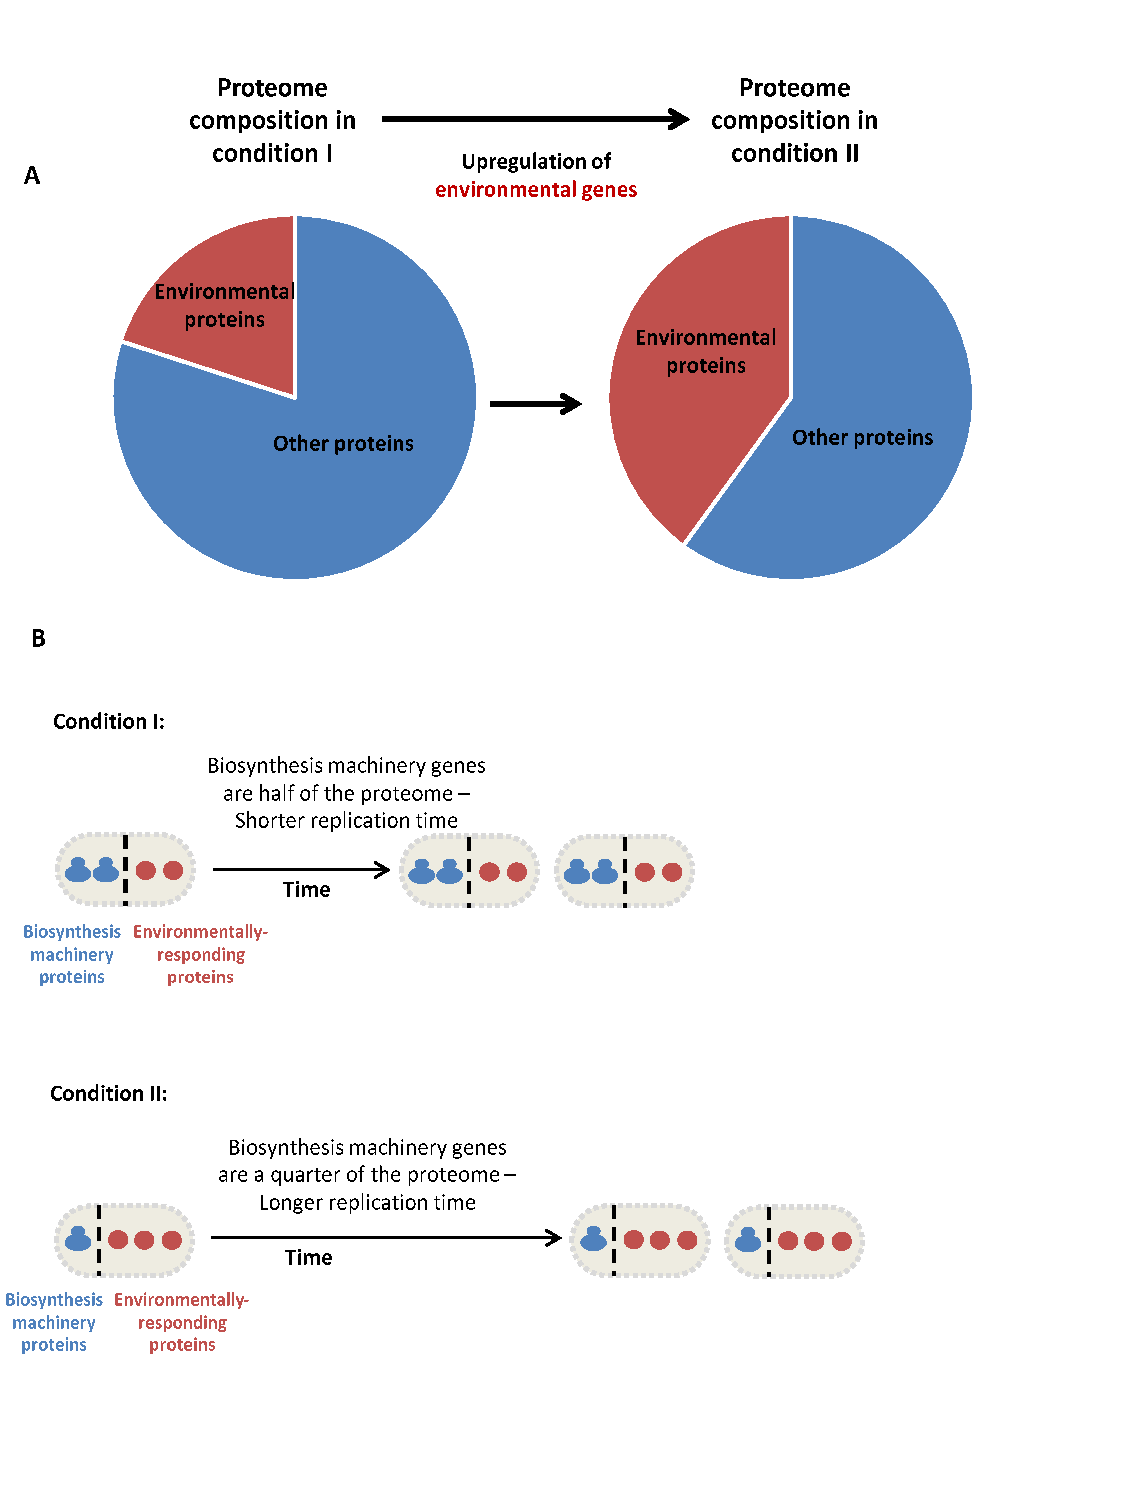
\includegraphics[scale=0.7]{Figures7-trieste.pdf}
\caption{
  A minimalistic model predicts down regulation of environmental genes increases the concentration of other proteins (Panel A).
As a result, the ratio of bio-synthesis machinery genes to the rest of the proteome increases, resulting in faster growth (Panel B).
}
\label{fig:model}
\end{figure}

\subsubsection{The concentration of a protein is determined by both gene specific control, and global expression machinery availability}
For every protein, the model separately considers the resulting concentration as the product of two control mechanisms:
\begin{enumerate}
\item Protein/gene specific controls such as the gene associated promoter sequence, 5'-UTRs, ribosomal binding site sequence, and factors affecting the specific expression of the gene such as transcription factors and riboswitches that react with the relevant gene.
  While some of these controls (such as, for example, the ribosomal binding sites) are static, and therefore condition independent, others are dynamic and may differ under different environmental conditions (such as transcription factors state).
\item The global availability of bio-synthetic resources in the cell, including availability of RNA Polymerase, co-factors, Ribosomes concentration, amino-acids etc.
  All of these factors can potentially differ across different environmental conditions.
\end{enumerate}
For simplicity, the model refers to the fraction of a specific protein out of the proteome, and not to the concentration of that protein in the biomass.
The concentration of a specific protein in the biomass can be calculated given this fraction and the concentration of total protein in the biomass, which is known to be relatively constant \cite{eco-sal,Scott2014} (for further discussion see \ref{protconc}).

According to the model, every gene, under every environmental condition, is given an 'affinity-for-expression' (or 'intrinsic-strength') score that encapsulates its gene-specific control state under the condition considered.
We denote the affinity of gene $i$ under growth condition $c$ by $w_i(c)$ (the notion of affinity for expression is not new, and was first suggested in  \cite{Maaloe1969}).
Our model assumes that the bio-synthetic resources of the cell (Ribosomes, RNA Polymerases, etc.) are distributed among the genes according to their affinities under the condition at hand.
The notion of affinities can thus reduce the number of parameters needed to predict expression levels markedly.
Instead of an expression level for every gene under each condition, there is only a need for the characterization of the affinities a gene may obtain under relevant environmental cues, a parameter set that is expected to be much smaller and easily characterized.
Figure \ref{fig:randpred} shows the prediction versus the actual concentration values of 9 random proteins in the data set from [ref Heinemann].

The resulting protein fraction, under a specific condition, is therefore its specific affinity under the condition, divided by the sum of all the affinities of all of the genes under that same condition.
Thus, if two proteins have the same affinity under some condition, they will occupy identical fractions out of the proteome under that condition.
If protein $A$ has twice the affinity of protein $B$ under a given condition, then the fraction $A$ occupies will be twice as large as the fraction occupied by $B$ under that condition, etc.

This relationship can be simply formulated as follows:
\begin{equation}
  \label{eq:concentration-ratio}
  p_i(c)=\frac{P_i(c)}{P(c)}=\frac{w_i(c)}{\sum_jw_j(c)}
\end{equation}
where $p_i(c)$ denotes the fraction of protein $i$ under condition $c$ out of the proteome, $P_i(c)$ denotes the mass of protein $i$ under condition $c$ per cell, $P(c)$ denotes the total mass of proteins per cell under condition $c$, and the sum, $\sum_jw_j(c)$, is taken over all the genes the cell has.

This equation implies that the observed fraction of a protein is determined by two factors, first, obviously, its own specific affinity that is present in the nominator, but second, and less intuitive and commonly thought of, the affinity of all of the other genes under the growth condition, as reflected by the denominator.

\subsubsection{A change in growth condition triggers changes in expression of specific proteins that indirectly affect all of the proteome}
Different environmental conditions may require the expression of different genes in order to achieve growth.
For example, comparing two growth media, one that includes amino-acids, and one that does not, it can be assumed that when amino-acids are present, no need exists for the cell to express amino-acids synthesizing enzymes, whereas when amino-acids are absent, these enzymes must be expressed.
Therefore, ideally, the cell will be able to sense the presence or absence of amino-acids in the growth media and, for the amino-acids synthesizing genes, down or up regulate their affinities accordingly.
If we now consider some arbitrary gene $i$, whose specific affinity is unaltered between these two conditions, we suggest that, other things being equal, its concentration will still change between the two conditions as the affinities of at least some of the other genes (the amino-acids synthesizing enzymes) change, changing the denominator in equation \ref{eq:concentration-ratio} and thus affecting the distribution of resources between all of the expressed genes.

Generalizing this notion, for every group of conditions, one could divide the proteins into those whose intrinsic affinity remains constant across all of the conditions, and to those whose intrinsic affinity changes (meaning their expression is actively regulated by the cell) between at least some of the conditions, as is shown in Figure \ref{fig:model}A.
An interesting consequence of the formulation in Equation \ref{eq:concentration-ratio} is that proteins whose intrinsic affinities remain constant across different growth conditions, also maintain their relative concentrations across these conditions with respect to each other.
Therefore, identifying a large group of proteins that maintain their relative concentrations across conditions (as was identified in section \ref{propchange}) may indicate that these proteins maintain their intrinsic affinities and that any changes in their absolute concentrations are in fact a passive outcome resulting from changes in the intrinsic affinities of other proteins.

\subsubsection{The observed growth rate is an outcome of proteome composition and environmental conditions}
While it is sometimes implied that different cellular components are regulated by the growth rate, here we consider the growth rate as an outcome of the environmental conditions that affect the proteome composition.
Specifically, we arrive at the doubling time as the result of dividing the total amount of proteins per cell by the amount of bio-synthesis machinery in that cell.
The larger the ratio of total proteins to bio-synthesis proteins is, the longer these bio-synthesis proteins will have to operate in order to duplicate the proteome, and thus the longer the doubling time of the cell will be.

To illustrate this assumption concretely, one could think about the total amount of proteins per cell (measured in amino-acids count) divided by the number of ribosomes in the cell.
Assuming each ribosome translates at an approximately condition-independent rate of about 20 amino-acids per second, and as the amount of actively translating ribosomes is also relatively condition-independent \cite{Philips2009}, it follows that the doubling time is linearly dependent on the ratio of proteins to ribosomes in the biomass as illustrated in Figure \ref{fig:model}B.

Theoretically, the fastest doubling time a cell may have is the doubling time achieved when all of the proteome of the cell is the bio-synthetic machinery.
We denote this minimal doubling time by $T_B$.
If the bio-synthetic machinery is only half of the proteome, the doubling time will be $2T_B$ etc.

To integrate the notion of total protein to bio-synthetic protein ratio into our model, we make the following simplifying assumption:
There is a group of bio-synthetic genes (e.g. genes of the transcriptional and translational machineries) the affinities of which remain constant across different growth conditions, a.k.a. these genes are not actively differentially regulated across different conditions.
Furthermore, we assume that the machineries these genes are involved at operate at relatively constant rates and active to non-active ratios across conditions.
Under these assumptions we can define this group of bio-synthesis genes, $G_B$, such that, for every gene that belongs to this group, $k \in G_B$, its affinity, $w_k(c)$ is constant regardless of the condition, $c$.
\begin{equation}
  \label{eq:biosynth-def}
  w_k(c)=w_k
\end{equation}

To keep our notations short, we will define the (condition independent) sum over all of these bio-synthesis genes as the constant: $W_B = \sum_{k\in G_B}w_k$.

As these genes form the bio-synthesis machinery, and according to the assumptions presented above, it follows that the doubling time under a given condition, $\tau(c)$ will be proportional to the ratio of total protein to bio-synthesis protein under that condition, with the proportionality constant being $T_B$:
\begin{equation}
  \label{eq:gr-ratio}
  \tau(c) = T_B\frac{P(c)}{\sum_{k\in G_B}P_k(c)}=T_B\frac{\sum_jw_j(c)}{W_B}
\end{equation}
Therefore, the model implies that for conditions that require the expression of larger amounts of non-bio-synthetic genes (i.e. higher values in the sum over $w_j$ that are not in $W_B$), the resulting doubling time will be longer, i.e., the growth rate will be lower.

\subsubsection{The concentration of a non-differentially regulated protein is expected to increase with the growth rate} 
Recalling that the connection between the growth rate and the doubling time is: $g(c)=\frac{\ln(2)}{\tau(c)}$, we now combine Equation \ref{eq:concentration-ratio} with Equation \ref{eq:gr-ratio} to get that:
\begin{equation}
  \label{eq:default-response}
  p_i(c)=\frac{w_i(c)}{\sum_jw_j(c)}=\frac{w_i(c)}{W_B}\frac{W_B}{\sum_jw_j(c)}=\frac{w_i(c)}{W_B}\frac{T_B}{\ln(2)}g(c)
\end{equation}

Incorporating all the condition-independent constants ($W_B$, $T_B$, $\ln(2)$) into one term, $C$, we get that the predicted fraction of protein $i$ out of the proteome under condition $c$ is:
\begin{equation}
  \label{eq:final-conc}
  p_i(c)=Cw_i(c)g(c)
\end{equation}
which implies that, for every two conditions between which gene $i$ maintains its affinity, ($w_i(c_1)=w_i(c_2)$), the fraction protein $i$ occupies out of the proteome scales like the growth rate change between these two conditions.

To summarize, the simplistic model we have constructed predicts that, under no specific regulation, the fraction a protein occupies out of the proteome should scale with the growth rate.
A group of such proteins should therefore maintain their relative concentrations across conditions.
Finally, when the growth rate approaches zero, the fractions of such proteins, and thus their concentrations, should also approach zero.

However, as the analysis of experimental data in Figure \ref{fig:globalgrcorr} shows, while the concentration of many proteins does indeed scale linearly with growth rate, this scaling does not imply a drop to zero concentration at zero growth.
There are at least two factors that have been neglected in the model, but that can account for this result, and the analysis of their expected effects follows.

\subsubsection{Protein degradation differentiates between measured growth rate and biomass synthesis rate}
Accounting for protein degradation affects the expected concentration of non-differentially regulated proteins at zero growth rate.
Thus, accounting for protein degradation may serve as a partial explanation for the discrepancy between experimental data and predictions made by the model.

Assuming that protein degradation acts on all proteins in the same way, and that it is invariant in the growth condition, the effect of protein degradation can be understood as follows: at any time, some fraction of the entire proteome is degraded.
Therefore, the \emph{observed} growth rate, $g$, is, in fact, the amount of proteins produced \emph{minus} the amount of proteins degraded.
To illustrate, if the measured growth rate is zero, the implication is not that no proteins are produced, but rather that proteins are produced at exactly the same rate as they are degraded.

Integrating this notion into the model means that, where the equations previously referred to the observed growth rate, $g$, as the indicator of protein synthesis rate, they should in fact refer to the observed growth rate plus the degradation rate, as that is the real rate of protein synthesis.
Therefore, if we denote by $\alpha$ the degradation rate (assuming for now equal degradation rates for all genes and under all conditions), Equation \ref{eq:final-conc} should be rewritten as:
\begin{equation}
  \label{eq:final-conc-deg}
  p_i(c)=Cw_i(c)(\alpha+g(c))
\end{equation}
This equation yields better agreement with the experimental results as presented in Figure \ref{fig:globalgrcorr}, depending on the exact value set for degradation.
Degradation can thus explain why the concentration of non-differentially regulated proteins does not drop to zero when the growth rate is zero.
The actual values obtained for the data analyzed are $\alpha=0.34$ for \cite{Valgepea2013} and $\alpha=0.52$ for \cite{Heinemann2014}, corresponding to protein half lives times of $T_{\text{deg}}=2$ hours and $T_{\text{deg}}=1.3$ hours respectively.
As these values correspond to relatively short half lives times, protein degradation is probably only a partial explanation for the differences between the predictions of the model and the observations obtained from the experimental data.

\subsubsection{Slower biological processes rates at slower growth affect the relation between proteome composition and growth rate}
The simplistic model assumes that the doubling time is proportional to the ratio of total protein to bio-synthetic protein.
This assumption fails if the rate at which the bio-synthetic machinery operates changes across conditions.
Replacing this assumption by a dependence of bio-synthesis rate with growth rate (such that, the faster the growth, the faster the synthesis rates), will affect the resulting predictions as well.
Slower bio-synthesis rates under slower growth rates imply that, compared with the model prediction, higher fraction of bio-synthesis proteins is needed to achieve a given growth rate.
Thus, lower synthesis rates under slower growth rates will be reflected by a lower slope and higher interception point for non-regulated proteins than those predicted by the model, as is indeed the case in Figure \ref{fig:globalgrcorr}.
\section{Future plans}
Despite the development of various whole proteome measurement techniques in recent years, very few data sets for \emph{E.Coli} have been published.
As such data sets are essential in order to answer systems-level physiological questions, my main future aim is to collect further data on the proteome of \emph{E.Coli} under various growth conditions.
To that end, we are currently building a chemostat/turbidostat system that will enable us to cultivate up to 8 cultures in dedicated containers as sources for exponentially growing cultures.
We are currently assessing two methods for measuring the proteome composition of such cultures, namely, mass spectrometry and ribosome profiling.
Our goal is to construct a data set that will include $10-20$ environmental conditions spanning various growth rates and carbon sources, each of which will be measured as a triplicate to assess biological and measurement errors.

Once the data is collected we aim to use it to address the following research questions:
1. Dispute or validate our assumptions regarding the extent of passive redistribution effects being a dominant effector on proteome composition.
2. Assess the variability in the proteome across conditions and compare it with the variability in cell size and macro-molecular composition.
3. Investigate the changes in enzyme efficiencies and apparent catalytic rates across conditions and their inter-dependence with the growth rate.
\end{document}
